\chapter{Idémyldring}
I dette steget i prosessen er målet å generere en liste over det vi tror kan være mulige årsaker til problemet. Det er en del forskjellige verktøy en kan bruke for å oppnå dette, men vi har valgt å benytte Idémyldring på bakgrunn av verktøyets egenskap til å generere mange idéer hurtig.

\section{Idémyldring}
I rotårsaksanalyse finnes det to ulike måter å gjennomføre Idémyldring på, Strukturert- og Ustrukturert Idémyldring. I den strukturerte versjonen får hver deltaker sin tur til å komme med en idé, og dette sikrer at alle får delta like mye. På den ustrukturerte måten kan alle komme med idéer når de dukker opp, og fungerer mye mer spontant enn den strukturelle. Det er spesielt viktig å ikke omformulere eller diskutere forslagene etterhvert som de kommer, dette skal gjøres etter Idémyldringsøkten er over.

\subsection{Ønsket utbytte}
Ønsket utbytte ved å bruke idémyldring her var for å få en forståelse av hva som kan være rotårsaken til at folk sine kontoer blir kompromittert.

\subsection{Gjennomførelse}
Det første som ble gjort når økten startet var å kommunisere og skrive opp problemstillingen på en tavle. Vi valgte å strukturere Idémyldringen som et tankekart ettersom dette var en kjent løsning for gruppen, og brukte den ustrukturerte tilnærmingen til Idémyldringen på grunn av dens uformelle og spontane natur. 

Problemet vi diskuterte og prøvde å komme med mulige måter folk kan kompromittere brukerkontoer til de ansatte ved skolen.

\subsection{Resultater}
Etter øktene var ferdig ble det gjort en vurdering av resultatene og de ble kategorisert i henhold til likhetstrekk, under en fellesnevner som for eksempel sosial manipulasjon. Resultater og gruppering er som vist i \hyperref[fig:idemyldring]{Figur 1} under.

\begin{figure}[H]
    \centering
    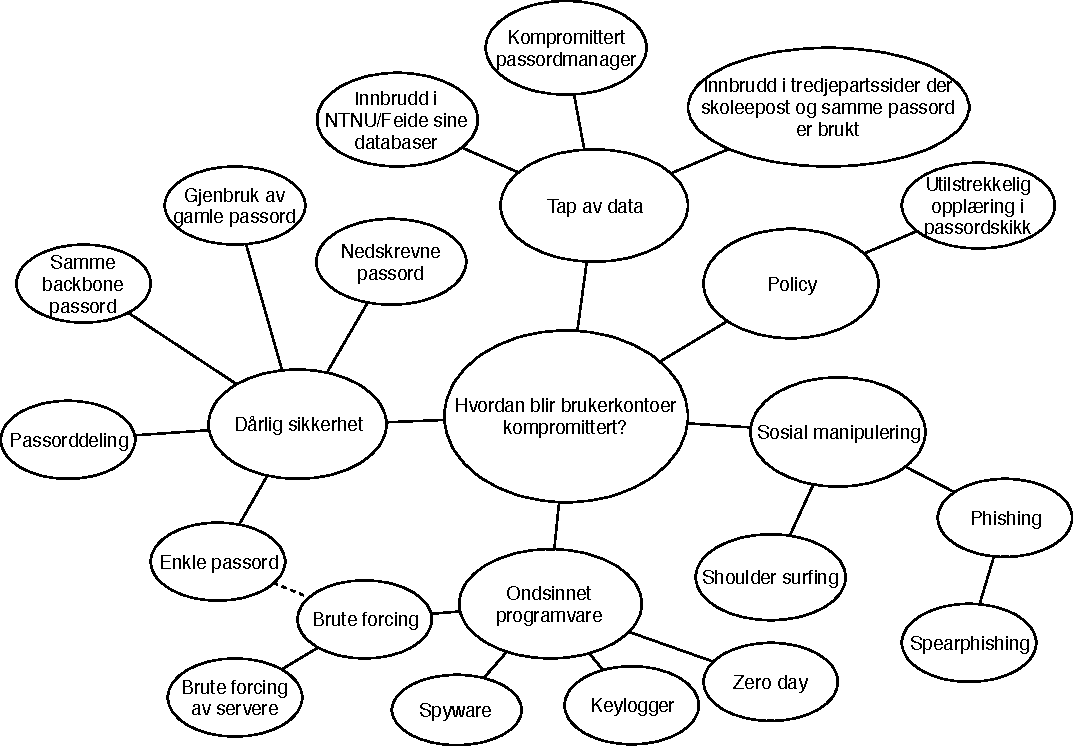
\includegraphics[scale=0.7]{case_2/bilder/idemyldring}
    \label{fig:idemyldring}
    \caption[Idémyldring]{Resultater og gruppering av idémyldringen}
\end{figure}

Resultatene er gruppert inn i 4 hoverkategorier;
\begin{description}
    \item[Dårlig sikkerhet] her er alt fra enkle passord til passordgjennbruk.
    \item [Tap av data] sider som dropbox har en lekkasje av brukere.
    \item[Sosial manipulering] 
    \item [Ondsinnet programmvare] programmvare, brukt som hjelpemiddel for å få tak i brukerinformasjon.
\end{description}
Merk 
\subsection{Konklusjon av verktøyet}
Dette var et effektivt verktøy for å få en overordnet oversikt over hva årsakene til at brukerkontoer blir kompromittert og grunner til at passord og brukernavn kan være på avveie